\documentclass[]{article}

\usepackage[utf8]{inputenc}
\usepackage{amsmath}
\usepackage{amssymb}
\usepackage{amsthm}
\usepackage{amsfonts}
\usepackage{graphicx}
\usepackage{capt-of}
\usepackage{listings}
\usepackage{siunitx}
\usepackage[section]{placeins}
\usepackage{float}



% Oppgavenummerering %
\renewcommand\thesection{Problem \arabic{section}}
\renewcommand\thesubsection{\alph{subsection})}

% Bevis
\newcommand\TombStone{\rule{.5em}{.5em}}
\renewcommand\qedsymbol{\TombStone}
\renewcommand{\proofname}{Bevis.} % Norske bevis

\title{}
\author{Sigurd Totland | MTTK}

\begin{document}
\maketitle

\section{4.9 I\&S}
\subsection{}
We recognize this system as a classic mass spring damper system. We obtain the given behaviour,
\begin{equation}\begin{aligned}
\label{eq:sys}
m \ddot y + \beta \dot y + k y = u,
\end{aligned}\end{equation}
or
\begin{equation}\begin{aligned}
m \ddot y = u -\beta \dot y - k y,
\end{aligned}\end{equation}
from newtons second law, i.e.
\begin{equation}\begin{aligned}
m \ddot y = F
\end{aligned}\end{equation}
where $F$ is the sum of all forces acting on the system. Inserting the dynamics for a spring, i.e. Hookes law,
\begin{equation}\begin{aligned}
F_1 = ky
\end{aligned}\end{equation}
and the dynamics of a damper,
\begin{equation}\begin{aligned}
F_2 = \beta \dot y,
\end{aligned}\end{equation}
as well as the input force $u$, we obtain the dynamics in \eqref{eq:sys}.

\subsection{}
We use the simple gradient algorithm with instantanious cost from I\&S. Table 4.2 summarizes it nicely,
\begin{align}
\label{eq:adaptive_law}
z = \theta^{*\top}\phi, \\
\hat z = \theta^\top \phi, \\
\epsilon = z - \hat z
\end{align}
where we have let the normalization term $m^2 = 1 - n_s^2 = 1$.
We rewrite the MSD system to state space form,
\begin{equation}\begin{aligned}
\dot x = Ax + b
\end{aligned}\end{equation}
where
\begin{equation}\begin{aligned}
A =
\begin{bmatrix}
0 & 1 \\
-\frac{k}{m} & -\frac{\beta}{m} \\
\end{bmatrix}, \quad
b = \begin{bmatrix}
0\\
\frac{1}{m}\\
\end{bmatrix}.
\end{aligned}\end{equation}
Using the same derivation as in assignment 2, the adaptive law in \eqref{eq:adaptive_law} becomes
\begin{equation}\begin{aligned}
\frac{1}{\Lambda(s)}u = \theta^{*\top}\frac{\alpha_2(s)}{\Lambda(s)}x.
\end{aligned}\end{equation}
where we choose $\Lambda$ to be a Hurwitz polynomial of order two, i.e. $\Lambda(s) = s^2 + \lambda_1 s + \lambda_0$.

\setcounter{subsection}{3}
\subsection{}
Using the starter code we simulate the system.
The simulation yields the following results (figure \ref{fig:results}). As we see, we are able to converge to the correct parameters.
\begin{figure}[H]
\centering
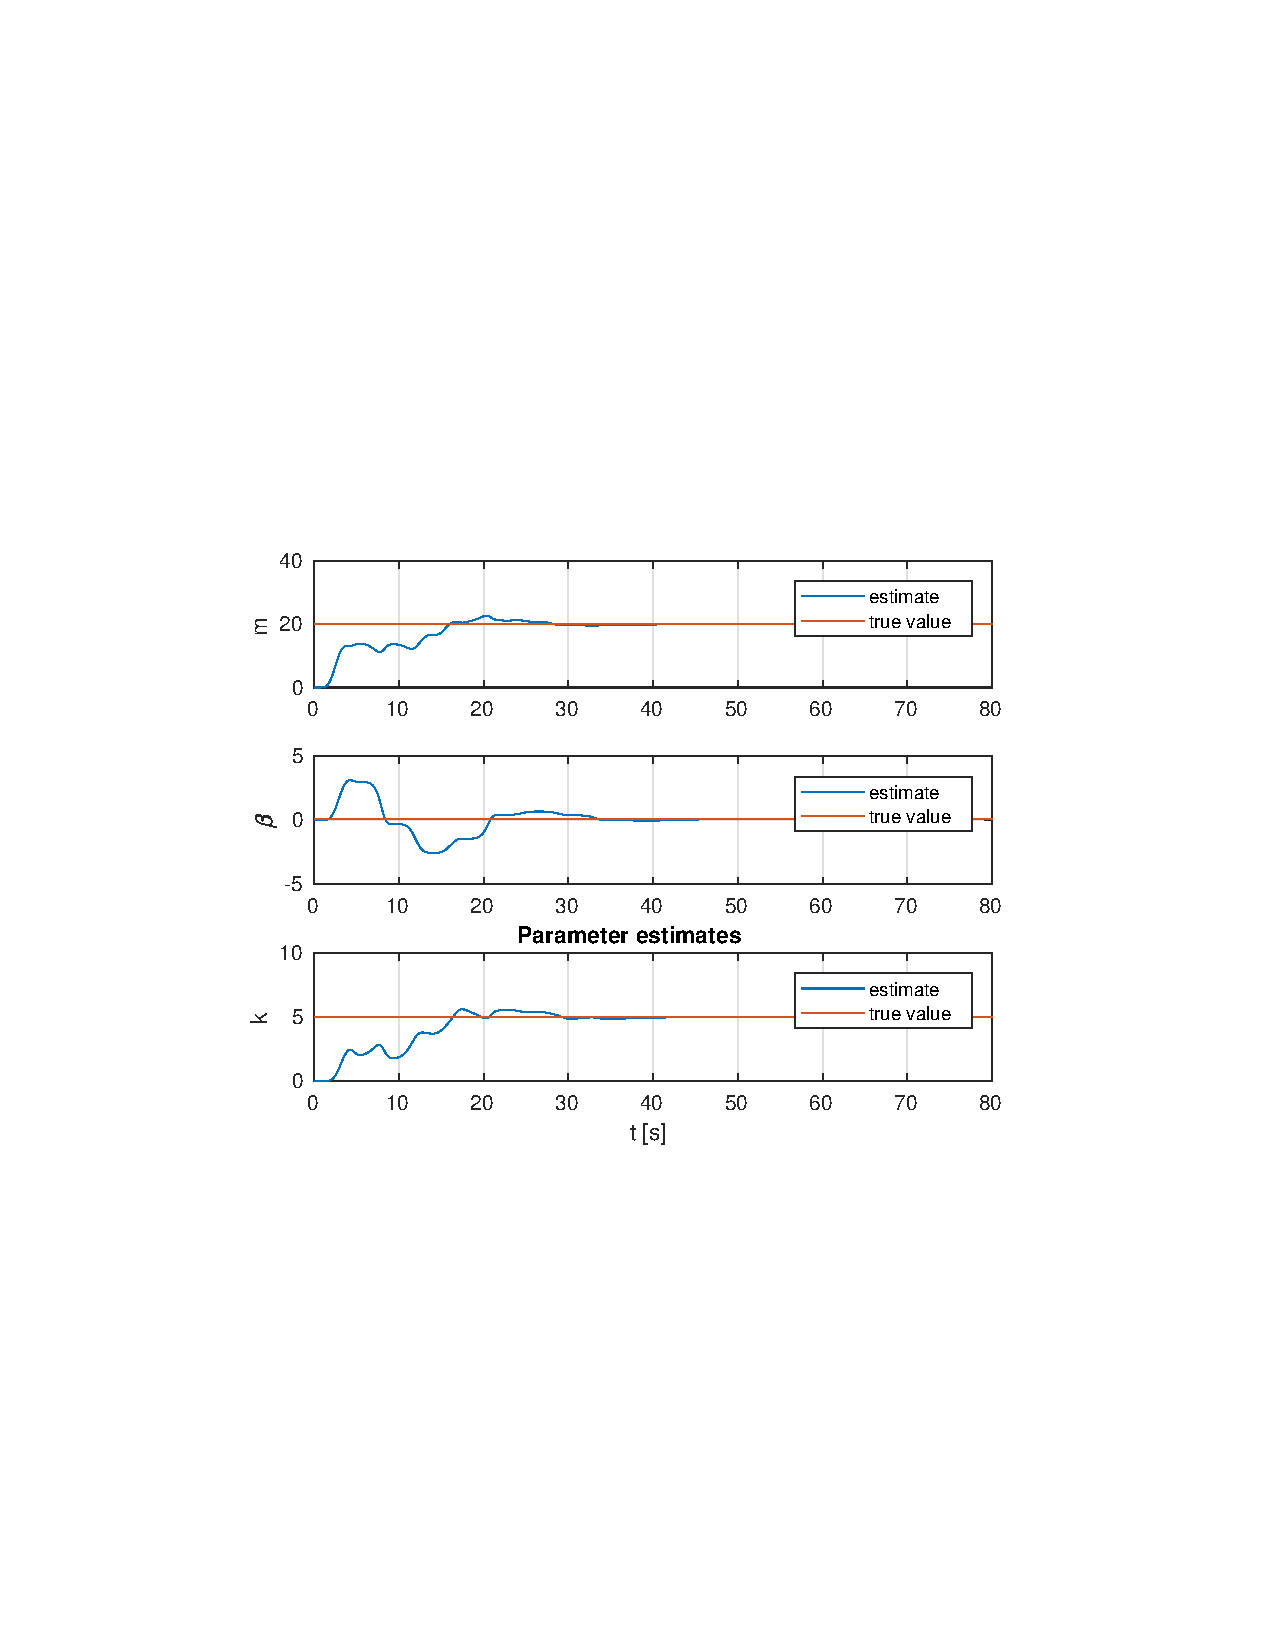
\includegraphics[width=0.3\textwidth, trim={8cm 8cm 8cm 8cm, clip}]{plots}
\caption{Parameter convergence with gradient method and instantaneous cost}
\label{fig:results}
\end{figure}

We then implement the integral cost function in our gradient descent method, that is we now have
\begin{align}
\dot \theta = -\Gamma (R \theta + Q), \\
\dot R = -\beta R + \frac{\phi \phi^\top}{m^2}, \quad R(0) = 0, \\
\dot Q = -\beta Q - \frac{z \phi}{m^2}, \quad Q(0) = 0,
\end{align}
When simulated, this results in the convergence shown in figure \ref{fig:int_results}.
\begin{figure}[H]
\centering
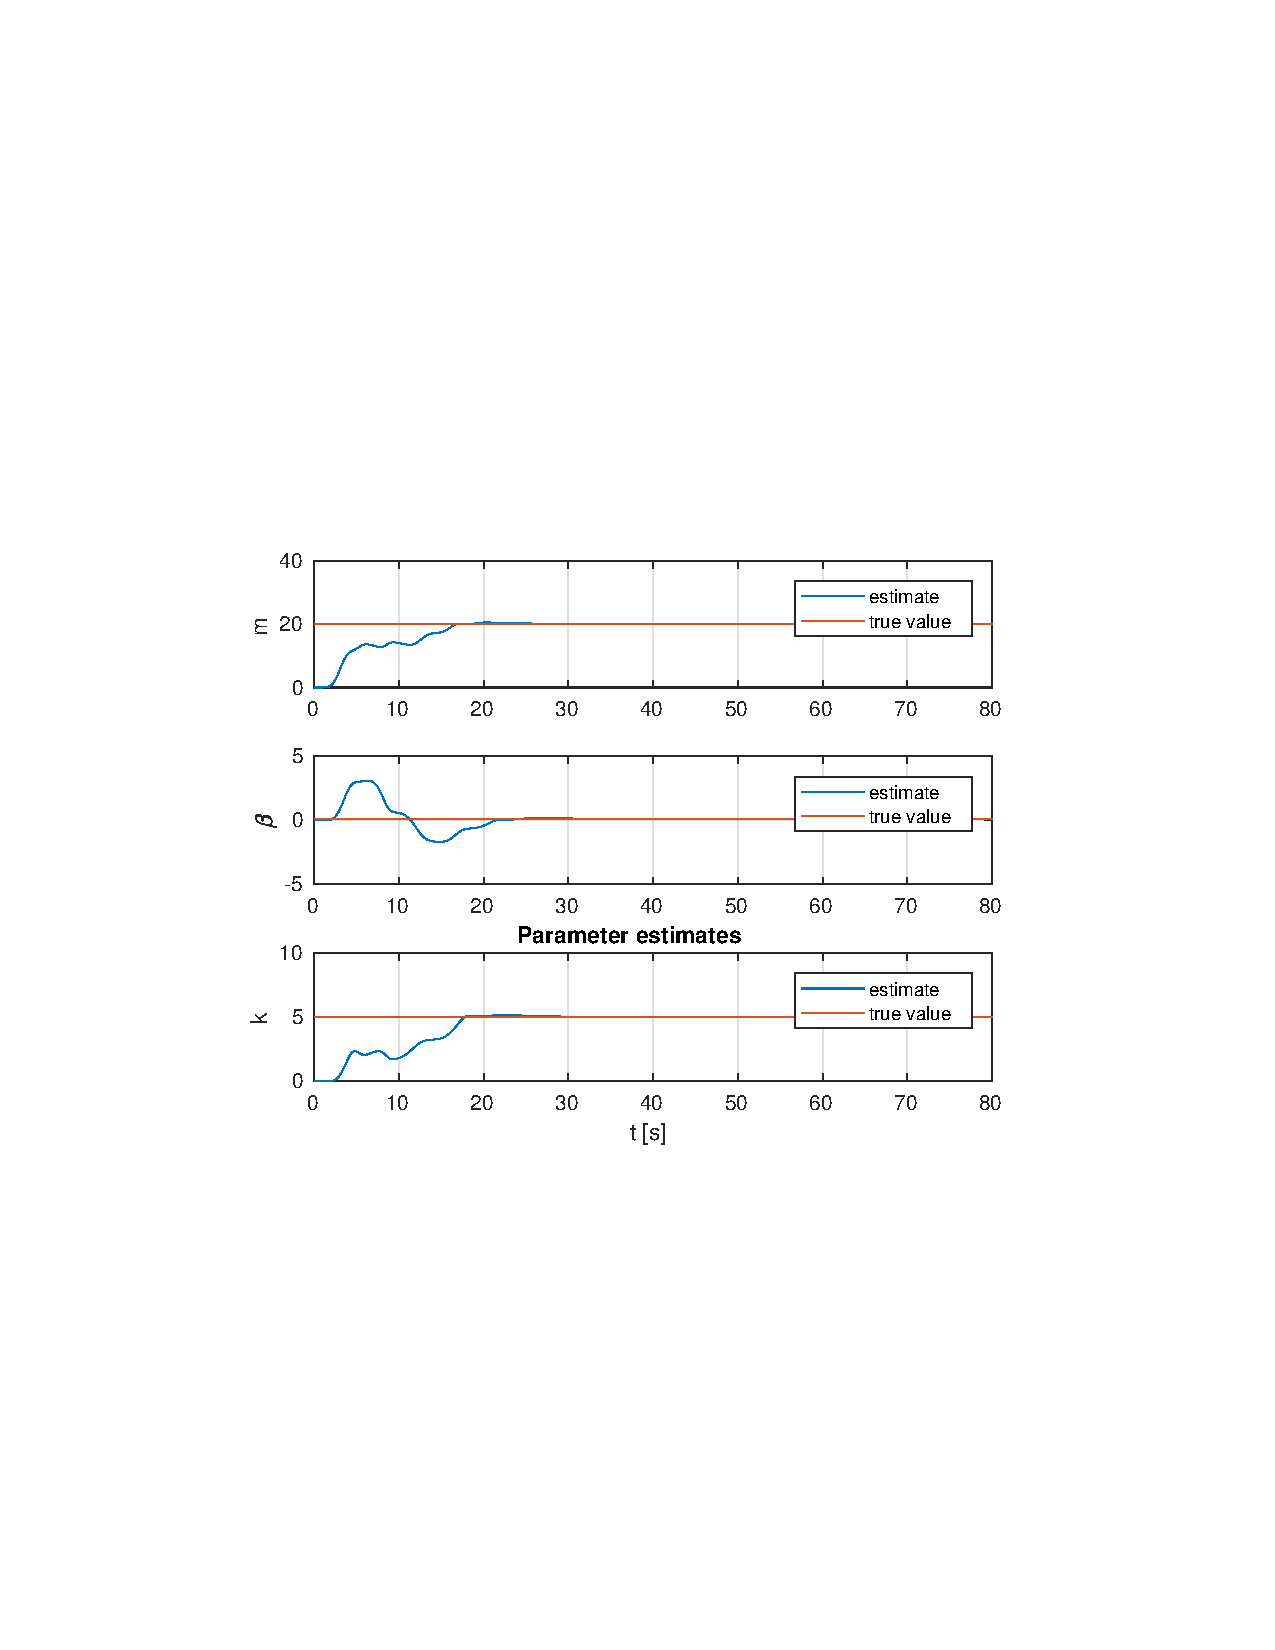
\includegraphics[width=0.3\textwidth, trim={8cm 8cm 8cm 8cm, clip}]{int_plots}
\caption{Parameter convergence with gradient method and integral cost}
\label{fig:int_results}
\end{figure}
As we can see, with the integral cost function, the system converges to the correct parameters a little faster.

\subsection{}
For this part, we make the mass time varying according to
\begin{equation}\begin{aligned}
m(t) = 20(2 - e^{-0.01(t-20)})
\end{aligned}\end{equation}
\begin{figure}[H]
\centering
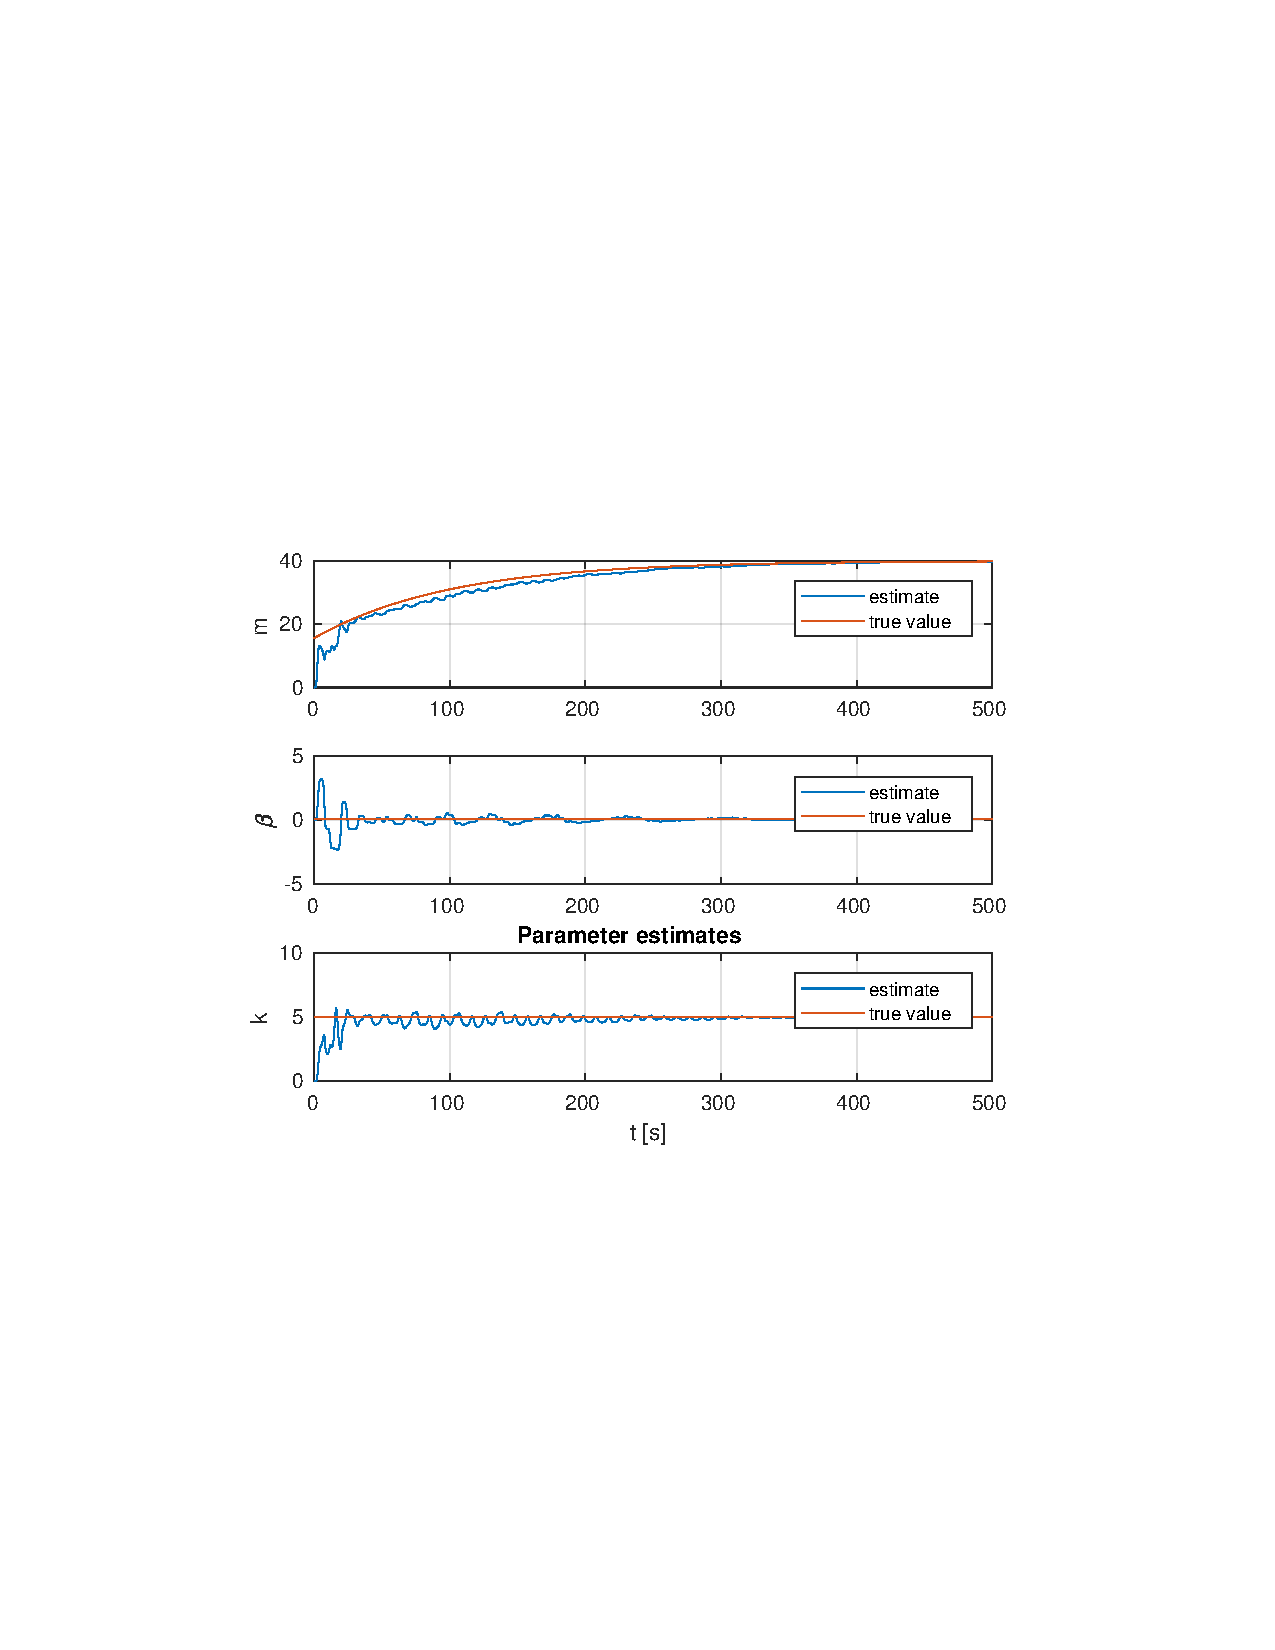
\includegraphics[width=0.3\textwidth, trim={8cm 8cm 8cm 8cm, clip}]{time_var_m}
\caption{Parameter convergence with time varying mass and instantaneous cost function gradient descent}
\label{fig:time_var_m}
\end{figure}
In figure \ref{fig:time_var_m} we see that the estimated parameters still converge to the actual, even when they are time varying. This does however invalidate the mathematical convergence proof that we have for the gradient method. This is due to an assumption in the Lyapunov analysis. When setting up the lyapunov ufunction, we assume the parameters, $\theta^{*}$, to be non-varying. It follows that the derivative of the parameter estimation error, $\tilde \theta = \frac{d}{dt}(\theta - \theta^*) = \dot \theta$ because $\dot \theta^* = 0$. When this value is non-zero however, the assumption breaks down, and the convergence guarantees no longer hold.

\end{document}

